\chapter{Appendix}
\clearpage

\section{Declaration of Authorship} \label{Declaration of Authorship}
We hereby certify that the thesis we are submitting is entirely our own original work except where otherwise indicated.
We are aware of the University's regulations concerning plagiarism, including those regulations concerning disciplinary actions that may result from plagiarism.
Any use of the works of any other author, in any form, is properly acknowledged at their point of use.
Furthermore, we would like to disclose that we have utilized the assistance of ChatGPT, an artificial intelligence language model developed by OpenAI,
to improve the clarity and coherence of the text. While ChatGPT has provided suggestions and refinements,
the overall content, ideas and analysis presented in this thesis remain our own.

\bigskip
\textbf{Location, Date} \\
Rapperswil, 24. January 2024

\vspace{1.2cm}
\begin{tabular}{@{}p{0.1cm}p{6cm}p{0.6cm}p{6cm}@{}}
	 & \hrulefill          &  & \hrulefill   \\ \\[-0.7em]
	 & Florian Baumgartner &  & Alain Keller \\
\end{tabular}


\includegraphics[width=4.8cm, align=t, smash=br, hshift=0.9cm, vshift=2.55cm]{appendix/Signature_Florian_Baumgartner.pdf}
\includegraphics[width=3.6cm, align=t, smash=br, hshift=8.25cm, vshift=1.8cm]{appendix/Signature_Alain_Keller.png}
\todo[inline]{Add Alain's signature here}
\newpage

\section{Data Archive} \label{Data Archive}
All created files and documents of this project are publicly available on GitHub. An institution called \textbf{PA-OST-2023} (\url{https://github.com/PA-OST-2023}) has been founded which contains repositories for each individual part of the project.
A quick description of the repositories including the associated web link is listed below:

\subsubsection{heron-administration} \vspace{-0.2cm}
\begin{description}
	\item[Description:] This repository contains all confidential information of the project.\vspace{-0.25cm}
	\item[URL:] \url{https://github.com/PA-OST-2023/heron-administration}\vspace{-0.25cm}
	\item[Type:] Private\vspace{-0.25cm}
\end{description}

\subsubsection{heron-literature} \vspace{-0.2cm}
\begin{description}
	\item[Description:] This repository contains all literature used in this project.\vspace{-0.25cm}
	\item[URL:] \url{https://github.com/PA-OST-2023/heron-literature}\vspace{-0.25cm}
	\item[Type:] Private\vspace{-0.25cm}
\end{description}

\subsubsection{heron-documentation} \vspace{-0.2cm}
\begin{description}
	\hfuzz=35.0pt
	\item[Description:] This repository contains this document.\vspace{-0.25cm}
	\item[URL:] \url{https://github.com/PA-OST-2023/heron-documentation}\vspace{-0.25cm}
	\item[Type:] Public\vspace{-0.25cm}
\end{description}

\subsubsection{heron-hardware} \vspace{-0.2cm}
\begin{description}
	\item[Description:] This repository contains hardware related documents (Schematics, PCB).\vspace{-0.25cm}
	\item[URL:] \url{https://github.com/PA-OST-2023/heron-hardware}\vspace{-0.25cm}
	\item[Type:] Public\vspace{-0.25cm}
\end{description}

\subsubsection{heron-firmware} \vspace{-0.2cm}
\begin{description}
	\item[Description:] This repository contains firmware source code written in C++.\vspace{-0.25cm}
	\item[URL:] \url{https://github.com/PA-OST-2023/heron-firmware}\vspace{-0.25cm}
	\item[Type:] Public\vspace{-0.25cm}
\end{description}

\subsubsection{heron-simulator} \vspace{-0.2cm}
\begin{description}
	\item[Description:] This repository contains the simulator source code written in Python.\vspace{-0.25cm}
	\item[URL:] \url{https://github.com/PA-OST-2023/heron-simulator}\vspace{-0.25cm}
	\item[Type:] Public\vspace{-0.25cm}
\end{description}

\subsubsection{heron-application} \vspace{-0.2cm}
\begin{description}
	\item[Description:] This repository contains the application source code written in Python.\vspace{-0.25cm}
	\item[URL:] \url{https://github.com/PA-OST-2023/heron-application}\vspace{-0.25cm}
	\item[Type:] Public\vspace{-0.25cm}
\end{description}

\subsubsection{heron-mechanical} \vspace{-0.2cm}
\begin{description}
	\item[Description:] This repository contains mechanical related documents (CAD-Files).\vspace{-0.25cm}
	\item[URL:] \url{https://github.com/PA-OST-2023/heron-mechanical}\vspace{-0.25cm}
	\item[Type:] Public\vspace{-0.25cm}
\end{description}

\subsubsection{heron-bastelstube} \vspace{-0.2cm}
\begin{description}
	\item[Description:] This repository contains temporary and experimental files.\vspace{-0.25cm}
	\item[URL:] \url{https://github.com/PA-OST-2023/heron-bastelstube}\vspace{-0.25cm}
	\item[Type:] Private\vspace{-0.25cm}
\end{description}
\newpage

\section{Definition of Task} \label{definition_of_task}
\enlargethispage{2.5cm}
\begin{adjustwidth}{0.23cm}{0cm} \hfuzz=7.0pt \vfuzz=19.0pt
	\makebox[\textwidth]{\frame{
\includegraphics[width=17.3cm, page=1]{appendix/Project_Definition_Audio_Localization.pdf}}}
\end{adjustwidth}
\newpage

\begin{adjustwidth}{-0.23cm}{0cm} \hfuzz=7.0pt \vfuzz=19.0pt
	\makebox[\textwidth]{\frame{
\includegraphics[width=17.3cm, page=2]{appendix/Project_Definition_Audio_Localization.pdf}}}
\end{adjustwidth}
\newpage

\section{Datasheet of MEMS Microphone (MP34DT05TR-A)} \label{appendix_datasheet_microphone}
\enlargethispage{2.5cm}
\begin{adjustwidth}{0.23cm}{0cm} \hfuzz=7.0pt \vfuzz=19.0pt
	\makebox[\textwidth]{\frame{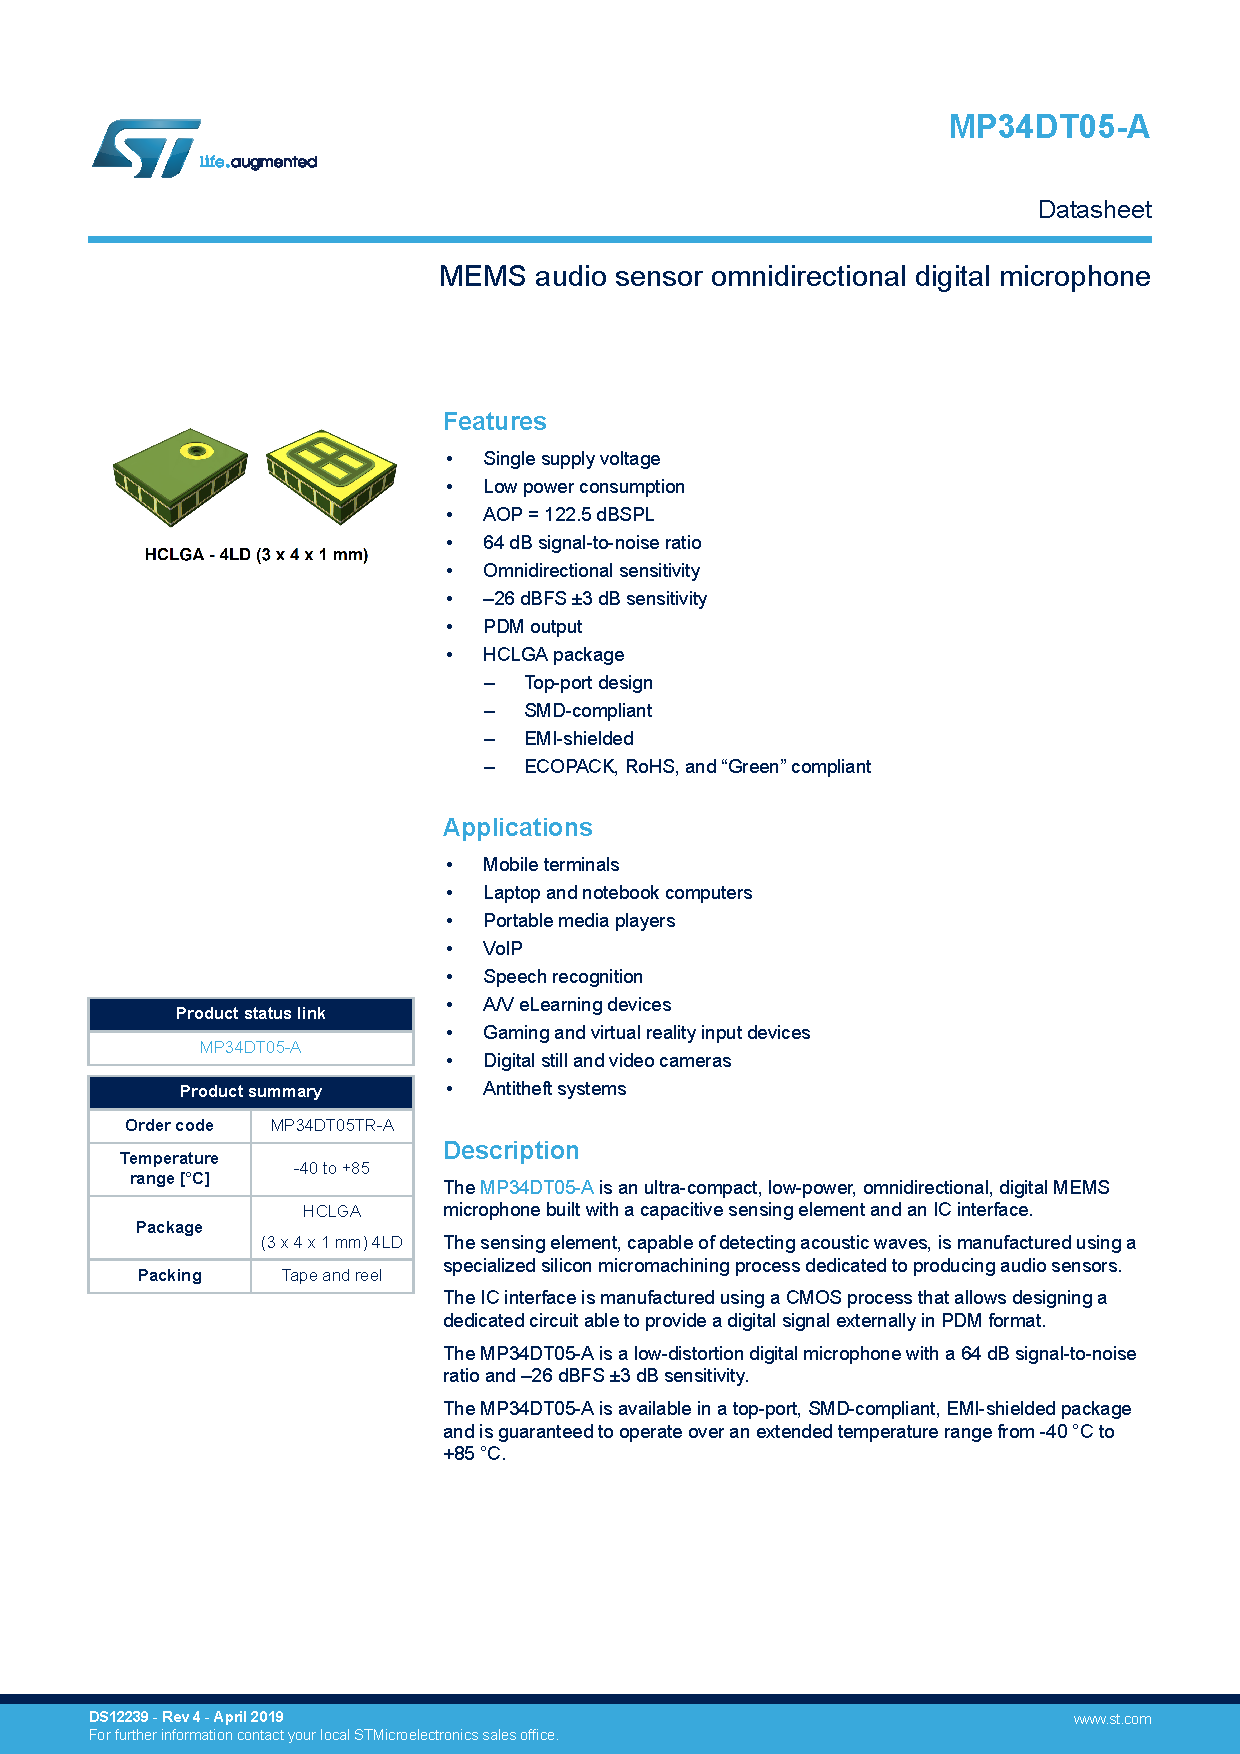
\includegraphics[angle=0, width=17.3cm, page=1]{appendix/Microphone_Datasheet.pdf}}}
\end{adjustwidth}
\newpage


\section{Microphone-Boards Schematics} \label{appendix_schematics_microphone_boards}
\enlargethispage{2.5cm}
\begin{adjustwidth}{-0.23cm}{0cm} \hfuzz=7.0pt \vfuzz=20.0pt
	\makebox[\textwidth]{\includegraphics[angle=90, width=17.3cm, page=1]{appendix/Microphone_Boards_V1.0.pdf}}
\end{adjustwidth}
\newpage

\begin{adjustwidth}{0.23cm}{0cm} \hfuzz=7.0pt \vfuzz=20.0pt
	\makebox[\textwidth]{\includegraphics[angle=90, width=17.3cm, page=2]{appendix/Microphone_Boards_V1.0.pdf}}
\end{adjustwidth}
\newpage

\begin{adjustwidth}{-0.23cm}{0cm} \hfuzz=7.0pt \vfuzz=20.0pt
	\makebox[\textwidth]{\includegraphics[angle=90, width=17.3cm, page=3]{appendix/Microphone_Boards_V1.0.pdf}}
\end{adjustwidth}
\newpage

\begin{adjustwidth}{0.23cm}{0cm} \hfuzz=7.0pt \vfuzz=20.0pt
	\makebox[\textwidth]{\includegraphics[angle=90, width=17.3cm, page=4]{appendix/Microphone_Boards_V1.0.pdf}}
\end{adjustwidth}
\newpage

\begin{adjustwidth}{-0.23cm}{0cm} \hfuzz=7.0pt \vfuzz=20.0pt
	\makebox[\textwidth]{\includegraphics[angle=90, width=17.3cm, page=5]{appendix/Microphone_Boards_V1.0.pdf}}
\end{adjustwidth}
\newpage

\section{Microphone-Boards PCB Top-Layer}
\enlargethispage{2.5cm}
\begin{adjustwidth}{0.23cm}{0cm} \hfuzz=7.0pt \vfuzz=19.0pt
	\makebox[\textwidth]{\includegraphics[angle=90, width=17.3cm, trim={0.3cm 0 0.3cm 0}, page=6]{appendix/Microphone_Boards_V1.0.pdf}}
\end{adjustwidth}
\newpage

\section{Microphone-Boards PCB Bottom-Layer}
\enlargethispage{2.5cm}
\begin{adjustwidth}{-0.23cm}{0cm} \hfuzz=7.0pt \vfuzz=19.0pt
	\makebox[\textwidth]{\includegraphics[angle=90, width=17.3cm, trim={0.3cm 0 0.3cm 0}, page=7]{appendix/Microphone_Boards_V1.0.pdf}}
\end{adjustwidth}
\newpage

\section{Microphone-Boards PCB Top-Overlay}
\enlargethispage{2.5cm}
\begin{adjustwidth}{0.23cm}{0cm} \hfuzz=7.0pt \vfuzz=19.0pt
	\makebox[\textwidth]{\includegraphics[angle=90, width=17.3cm, trim={0.3cm 0 0.3cm 0}, page=8]{appendix/Microphone_Boards_V1.0.pdf}}
\end{adjustwidth}
\newpage

\section{Microphone-Boards PCB Bottom-Overlay}
\enlargethispage{2.5cm}
\begin{adjustwidth}{-0.23cm}{0cm} \hfuzz=7.0pt \vfuzz=19.0pt
	\makebox[\textwidth]{\includegraphics[angle=90, width=17.3cm, trim={0.3cm 0 0.3cm 0}, page=9]{appendix/Microphone_Boards_V1.0.pdf}}
\end{adjustwidth}
\newpage

\section{Microphone-Boards PCB Outline}
\enlargethispage{2.5cm}
\begin{adjustwidth}{0.23cm}{0cm} \hfuzz=7.0pt \vfuzz=19.0pt
	\makebox[\textwidth]{\includegraphics[angle=90, width=17.3cm, trim={0.3cm 0 0.3cm 0}, page=10]{appendix/Microphone_Boards_V1.0.pdf}}
\end{adjustwidth}
\newpage

\section{Microphone-Boards Bill of Materials (BOM)}
\enlargethispage{2.5cm}
\begin{adjustwidth}{-0.23cm}{0cm} \hfuzz=7.0pt \vfuzz=20.0pt
	\vspace{0.2cm}
	\makebox[\textwidth]{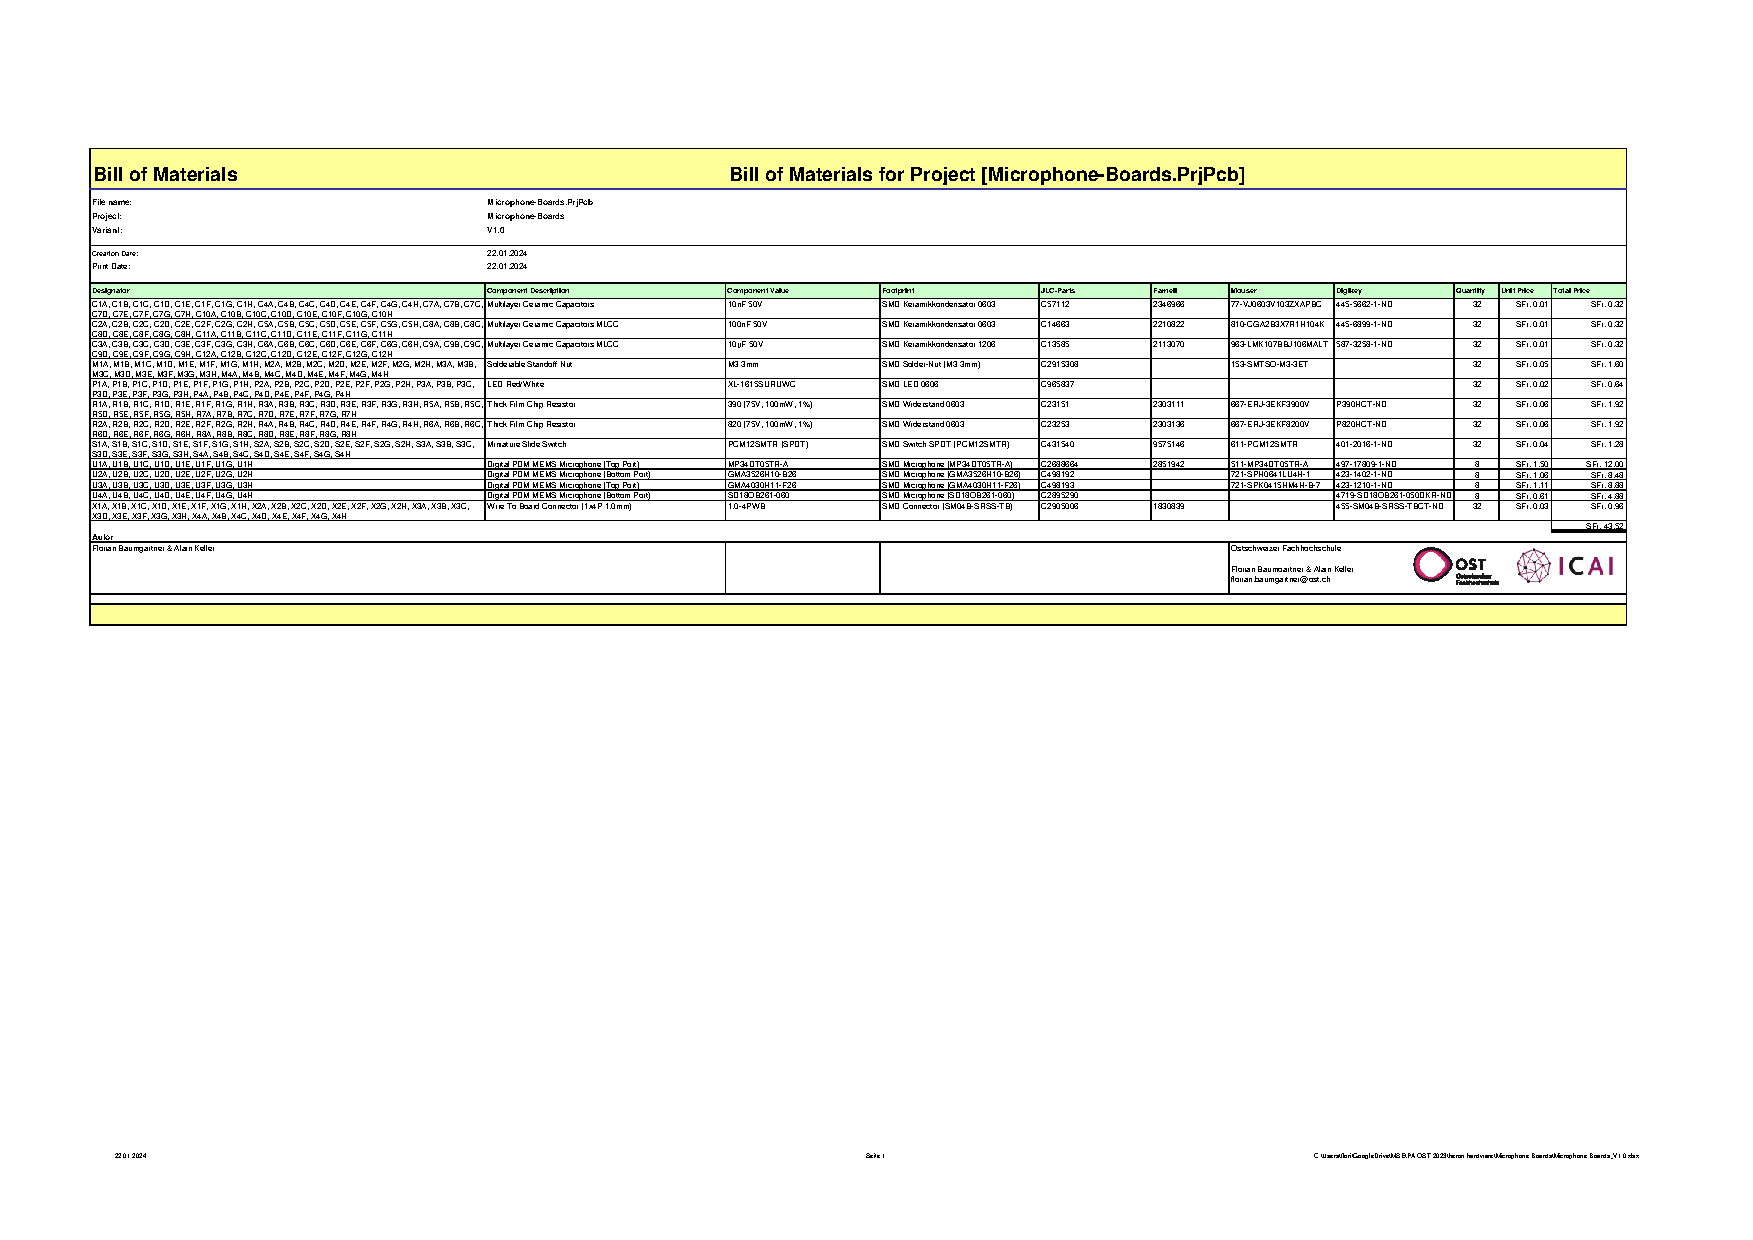
\includegraphics[angle=90, height=24.0cm]{appendix/Microphone_Boards_V1.0_BOM.pdf}}
\end{adjustwidth}
\newpage


\section{Acquisition-System Schematics} \label{appendix_schematics_acquisition_system}
\enlargethispage{2.5cm}
\begin{adjustwidth}{0.23cm}{0cm} \hfuzz=7.0pt \vfuzz=20.0pt
	\makebox[\textwidth]{\includegraphics[angle=90, width=17.3cm, page=1]{appendix/Acquisition_System_V1.0.pdf}}
\end{adjustwidth}
\newpage

\begin{adjustwidth}{-0.23cm}{0cm} \hfuzz=7.0pt \vfuzz=20.0pt
	\makebox[\textwidth]{\includegraphics[angle=90, width=17.3cm, page=2]{appendix/Acquisition_System_V1.0.pdf}}
\end{adjustwidth}
\newpage

\begin{adjustwidth}{0.23cm}{0cm} \hfuzz=7.0pt \vfuzz=20.0pt
	\makebox[\textwidth]{\includegraphics[angle=90, width=17.3cm, page=3]{appendix/Acquisition_System_V1.0.pdf}}
\end{adjustwidth}
\newpage

\begin{adjustwidth}{-0.23cm}{0cm} \hfuzz=7.0pt \vfuzz=20.0pt
	\makebox[\textwidth]{\includegraphics[angle=90, width=17.3cm, page=4]{appendix/Acquisition_System_V1.0.pdf}}
\end{adjustwidth}
\newpage

\begin{adjustwidth}{0.23cm}{0cm} \hfuzz=7.0pt \vfuzz=20.0pt
	\makebox[\textwidth]{\includegraphics[angle=90, width=17.3cm, page=5]{appendix/Acquisition_System_V1.0.pdf}}
\end{adjustwidth}
\newpage

\section{Acquisition-System PCB Top-Layer}
\enlargethispage{2.5cm}
\begin{adjustwidth}{-0.23cm}{0cm} \hfuzz=7.0pt \vfuzz=19.0pt
	\makebox[\textwidth]{\includegraphics[angle=90, width=17.3cm, trim={0.3cm 0 0.3cm 0}, page=6]{appendix/Acquisition_System_V1.0.pdf}}
\end{adjustwidth}
\newpage

\section{Acquisition-System PCB Mid-Layer 1}
\enlargethispage{2.5cm}
\begin{adjustwidth}{0.23cm}{0cm} \hfuzz=7.0pt \vfuzz=19.0pt
	\makebox[\textwidth]{\includegraphics[angle=90, width=17.3cm, trim={0.3cm 0 0.3cm 0}, page=7]{appendix/Acquisition_System_V1.0.pdf}}
\end{adjustwidth}
\newpage

\section{Acquisition-System PCB Mid-Layer 2}
\enlargethispage{2.5cm}
\begin{adjustwidth}{-0.23cm}{0cm} \hfuzz=7.0pt \vfuzz=19.0pt
	\makebox[\textwidth]{\includegraphics[angle=90, width=17.3cm, trim={0.3cm 0 0.3cm 0}, page=8]{appendix/Acquisition_System_V1.0.pdf}}
\end{adjustwidth}
\newpage

\section{Acquisition-System PCB Bottom-Layer}
\enlargethispage{2.5cm}
\begin{adjustwidth}{0.23cm}{0cm} \hfuzz=7.0pt \vfuzz=19.0pt
	\makebox[\textwidth]{\includegraphics[angle=90, width=17.3cm, trim={0.3cm 0 0.3cm 0}, page=9]{appendix/Acquisition_System_V1.0.pdf}}
\end{adjustwidth}
\newpage

\section{Acquisition-System PCB Top-Overlay}
\enlargethispage{2.5cm}
\begin{adjustwidth}{-0.23cm}{0cm} \hfuzz=7.0pt \vfuzz=19.0pt
	\makebox[\textwidth]{\includegraphics[angle=90, width=17.3cm, trim={0.3cm 0 0.3cm 0}, page=10]{appendix/Acquisition_System_V1.0.pdf}}
\end{adjustwidth}
\newpage

\section{Acquisition-System PCB Bottom-Overlay}
\enlargethispage{2.5cm}
\begin{adjustwidth}{0.23cm}{0cm} \hfuzz=7.0pt \vfuzz=19.0pt
	\makebox[\textwidth]{\includegraphics[angle=90, width=17.3cm, trim={0.3cm 0 0.3cm 0}, page=11]{appendix/Acquisition_System_V1.0.pdf}}
\end{adjustwidth}
\newpage

\section{Acquisition-System PCB Outline}
\enlargethispage{2.5cm}
\begin{adjustwidth}{-0.23cm}{0cm} \hfuzz=7.0pt \vfuzz=19.0pt
	\makebox[\textwidth]{\includegraphics[angle=90, width=17.3cm, trim={0.3cm 0 0.3cm 0}, page=12]{appendix/Acquisition_System_V1.0.pdf}}
\end{adjustwidth}
\newpage

\section{Acquisition-System Bill of Materials (BOM)}
\enlargethispage{2.5cm}
\begin{adjustwidth}{0.23cm}{0cm} \hfuzz=7.0pt \vfuzz=20.0pt
	\vspace{0.2cm}
	\makebox[\textwidth]{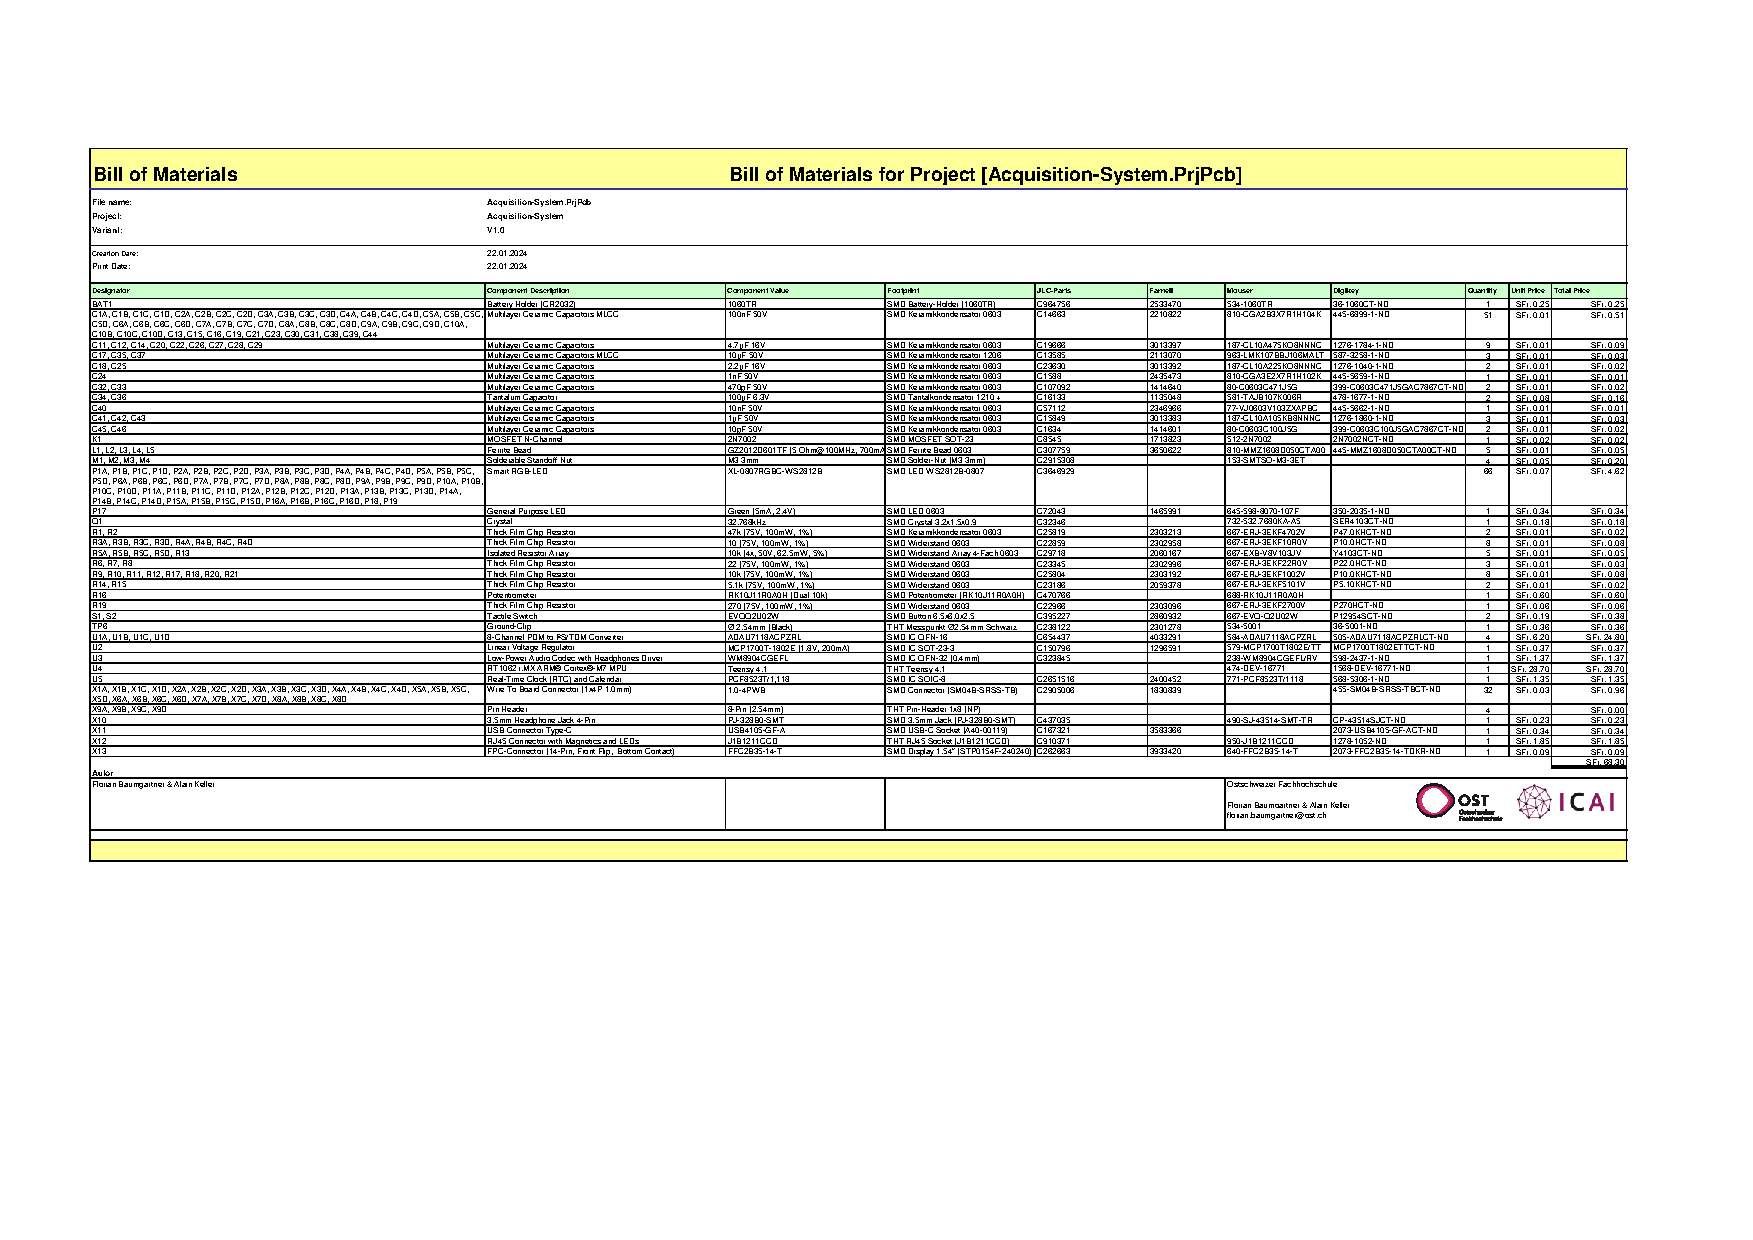
\includegraphics[angle=90, height=24.0cm]{appendix/Acquisition_System_V1.0_BOM.pdf}}
\end{adjustwidth}
\newpage



\section{Mainboard Schematics} \label{appendix_schematics_mainboard}
\enlargethispage{2.5cm}
\begin{adjustwidth}{-0.23cm}{0cm} \hfuzz=7.0pt \vfuzz=20.0pt
	\makebox[\textwidth]{\includegraphics[angle=90, width=17.3cm, page=1]{appendix/Mainboard_V1.0.pdf}}
\end{adjustwidth}
\newpage

\begin{adjustwidth}{0.23cm}{0cm} \hfuzz=7.0pt \vfuzz=20.0pt
	\makebox[\textwidth]{\includegraphics[angle=90, width=17.3cm, page=2]{appendix/Mainboard_V1.0.pdf}}
\end{adjustwidth}
\newpage

\begin{adjustwidth}{-0.23cm}{0cm} \hfuzz=7.0pt \vfuzz=20.0pt
	\makebox[\textwidth]{\includegraphics[angle=90, width=17.3cm, page=3]{appendix/Mainboard_V1.0.pdf}}
\end{adjustwidth}
\newpage

\begin{adjustwidth}{0.23cm}{0cm} \hfuzz=7.0pt \vfuzz=20.0pt
	\makebox[\textwidth]{\includegraphics[angle=90, width=17.3cm, page=4]{appendix/Mainboard_V1.0.pdf}}
\end{adjustwidth}
\newpage

\begin{adjustwidth}{-0.23cm}{0cm} \hfuzz=7.0pt \vfuzz=20.0pt
	\makebox[\textwidth]{\includegraphics[angle=90, width=17.3cm, page=5]{appendix/Mainboard_V1.0.pdf}}
\end{adjustwidth}
\newpage

\begin{adjustwidth}{0.23cm}{0cm} \hfuzz=7.0pt \vfuzz=20.0pt
	\makebox[\textwidth]{\includegraphics[angle=90, width=17.3cm, page=6]{appendix/Mainboard_V1.0.pdf}}
\end{adjustwidth}
\newpage

\begin{adjustwidth}{-0.23cm}{0cm} \hfuzz=7.0pt \vfuzz=20.0pt
	\makebox[\textwidth]{\includegraphics[angle=90, width=17.3cm, page=7]{appendix/Mainboard_V1.0.pdf}}
\end{adjustwidth}
\newpage

\section{Mainboard PCB Top-Layer}
\enlargethispage{2.5cm}
\begin{adjustwidth}{0.23cm}{0cm} \hfuzz=7.0pt \vfuzz=19.0pt
	\makebox[\textwidth]{\includegraphics[angle=90, width=17.3cm, trim={0.3cm 0 0.3cm 0}, page=8]{appendix/Mainboard_V1.0.pdf}}
\end{adjustwidth}
\newpage

\section{Mainboard PCB Mid-Layer 1}
\enlargethispage{2.5cm}
\begin{adjustwidth}{-0.23cm}{0cm} \hfuzz=7.0pt \vfuzz=19.0pt
	\makebox[\textwidth]{\includegraphics[angle=90, width=17.3cm, trim={0.3cm 0 0.3cm 0}, page=9]{appendix/Mainboard_V1.0.pdf}}
\end{adjustwidth}
\newpage

\section{Mainboard PCB Mid-Layer 2}
\enlargethispage{2.5cm}
\begin{adjustwidth}{0.23cm}{0cm} \hfuzz=7.0pt \vfuzz=19.0pt
	\makebox[\textwidth]{\includegraphics[angle=90, width=17.3cm, trim={0.3cm 0 0.3cm 0}, page=10]{appendix/Mainboard_V1.0.pdf}}
\end{adjustwidth}
\newpage

\section{Mainboard PCB Bottom-Layer}
\enlargethispage{2.5cm}
\begin{adjustwidth}{-0.23cm}{0cm} \hfuzz=7.0pt \vfuzz=19.0pt
	\makebox[\textwidth]{\includegraphics[angle=90, width=17.3cm, trim={0.3cm 0 0.3cm 0}, page=11]{appendix/Mainboard_V1.0.pdf}}
\end{adjustwidth}
\newpage

\section{Mainboard PCB Top-Overlay}
\enlargethispage{2.5cm}
\begin{adjustwidth}{0.23cm}{0cm} \hfuzz=7.0pt \vfuzz=19.0pt
	\makebox[\textwidth]{\includegraphics[angle=90, width=17.3cm, trim={0.3cm 0 0.3cm 0}, page=12]{appendix/Mainboard_V1.0.pdf}}
\end{adjustwidth}
\newpage

\section{Mainboard PCB Bottom-Overlay}
\enlargethispage{2.5cm}
\begin{adjustwidth}{-0.23cm}{0cm} \hfuzz=7.0pt \vfuzz=19.0pt
	\makebox[\textwidth]{\includegraphics[angle=90, width=17.3cm, trim={0.3cm 0 0.3cm 0}, page=13]{appendix/Mainboard_V1.0.pdf}}
\end{adjustwidth}
\newpage

\section{Mainboard PCB Outline}
\enlargethispage{2.5cm}
\begin{adjustwidth}{0.23cm}{0cm} \hfuzz=7.0pt \vfuzz=19.0pt
	\makebox[\textwidth]{\includegraphics[angle=90, width=17.3cm, trim={0.3cm 0 0.3cm 0}, page=14]{appendix/Mainboard_V1.0.pdf}}
\end{adjustwidth}
\newpage

\section{Mainboard Bill of Materials (BOM)}
\enlargethispage{2.5cm}
\begin{adjustwidth}{-0.23cm}{0cm} \hfuzz=7.0pt \vfuzz=20.0pt
	\vspace{0.2cm}
	\makebox[\textwidth]{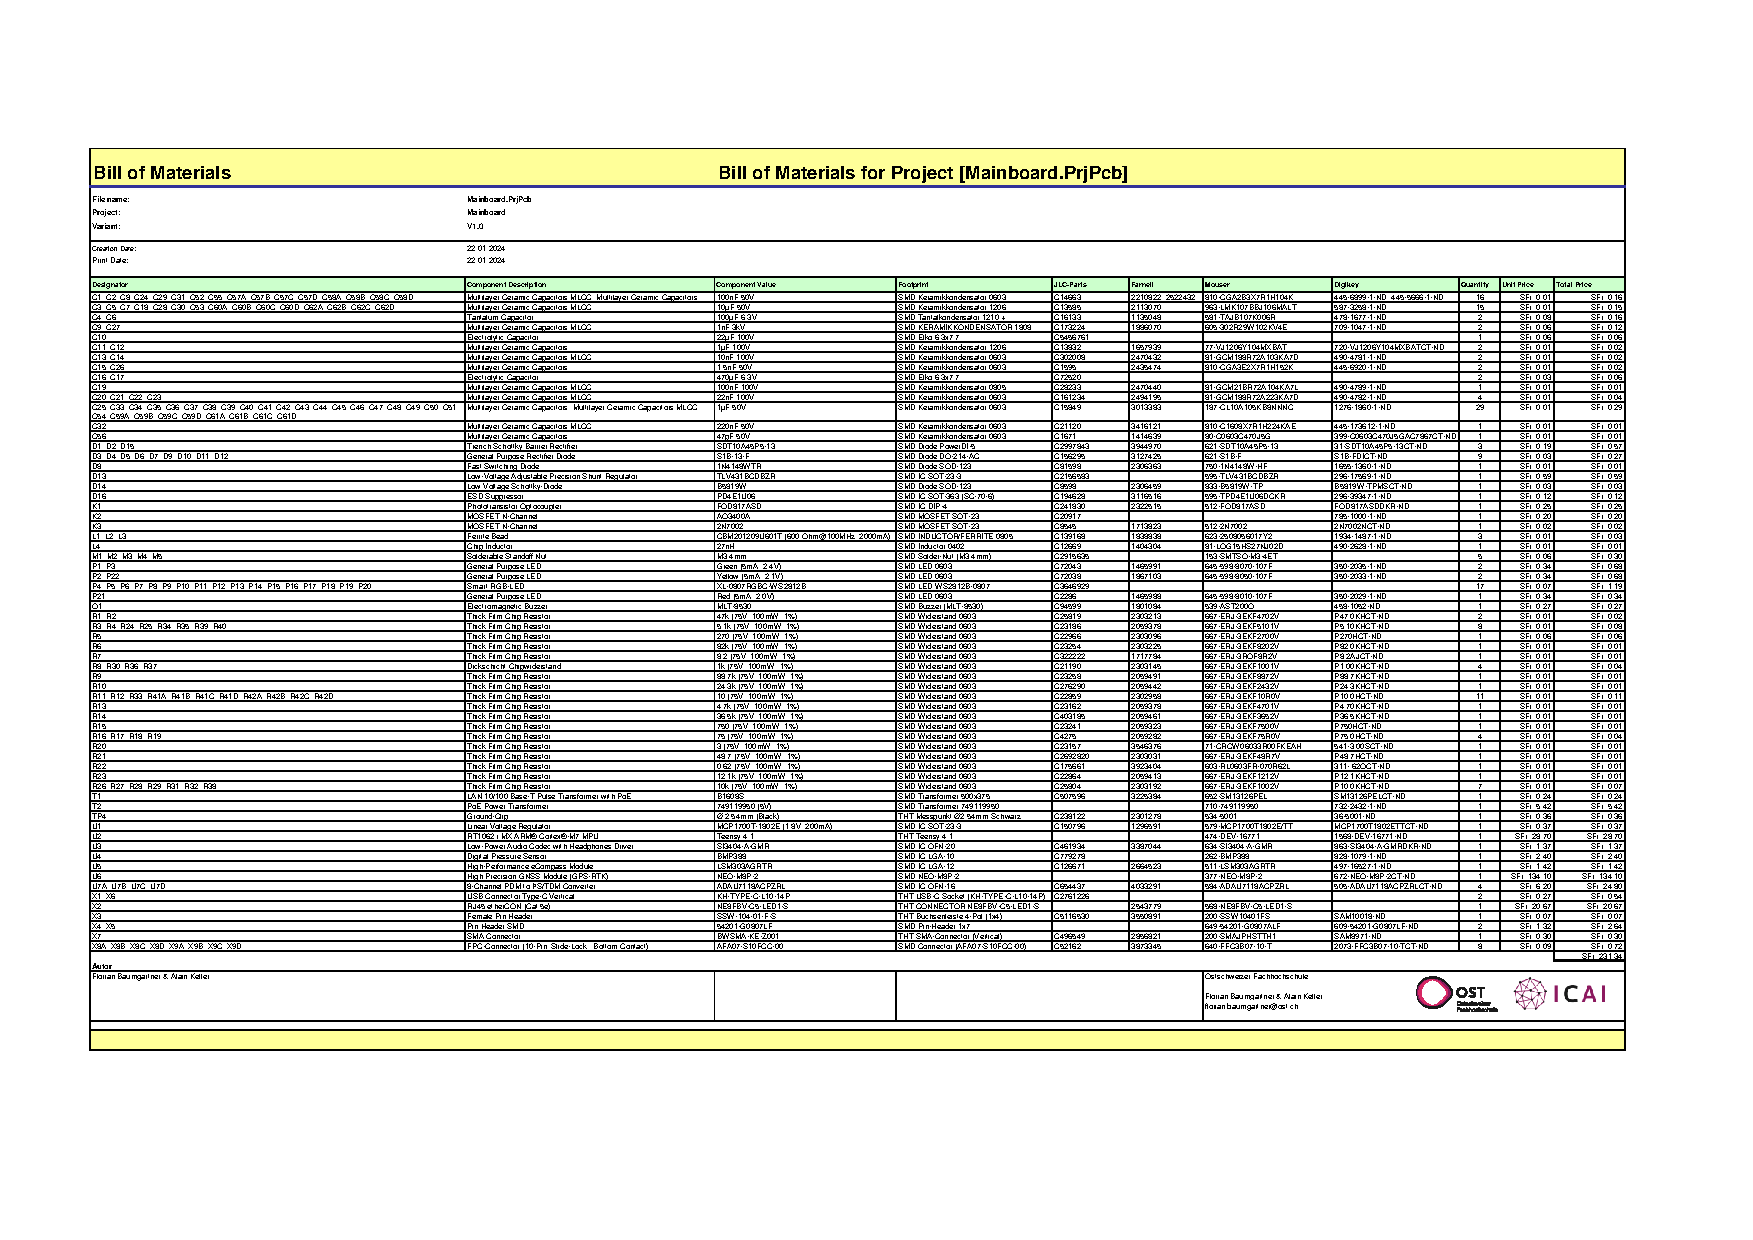
\includegraphics[angle=90, height=24.0cm]{appendix/Mainboard_V1.0_BOM.pdf}}
\end{adjustwidth}
\newpage



\section{Microphone-Arm Schematics} \label{appendix_schematics_microphone_arm}
\enlargethispage{2.5cm}
\begin{adjustwidth}{0.23cm}{0cm} \hfuzz=7.0pt \vfuzz=20.0pt
	\makebox[\textwidth]{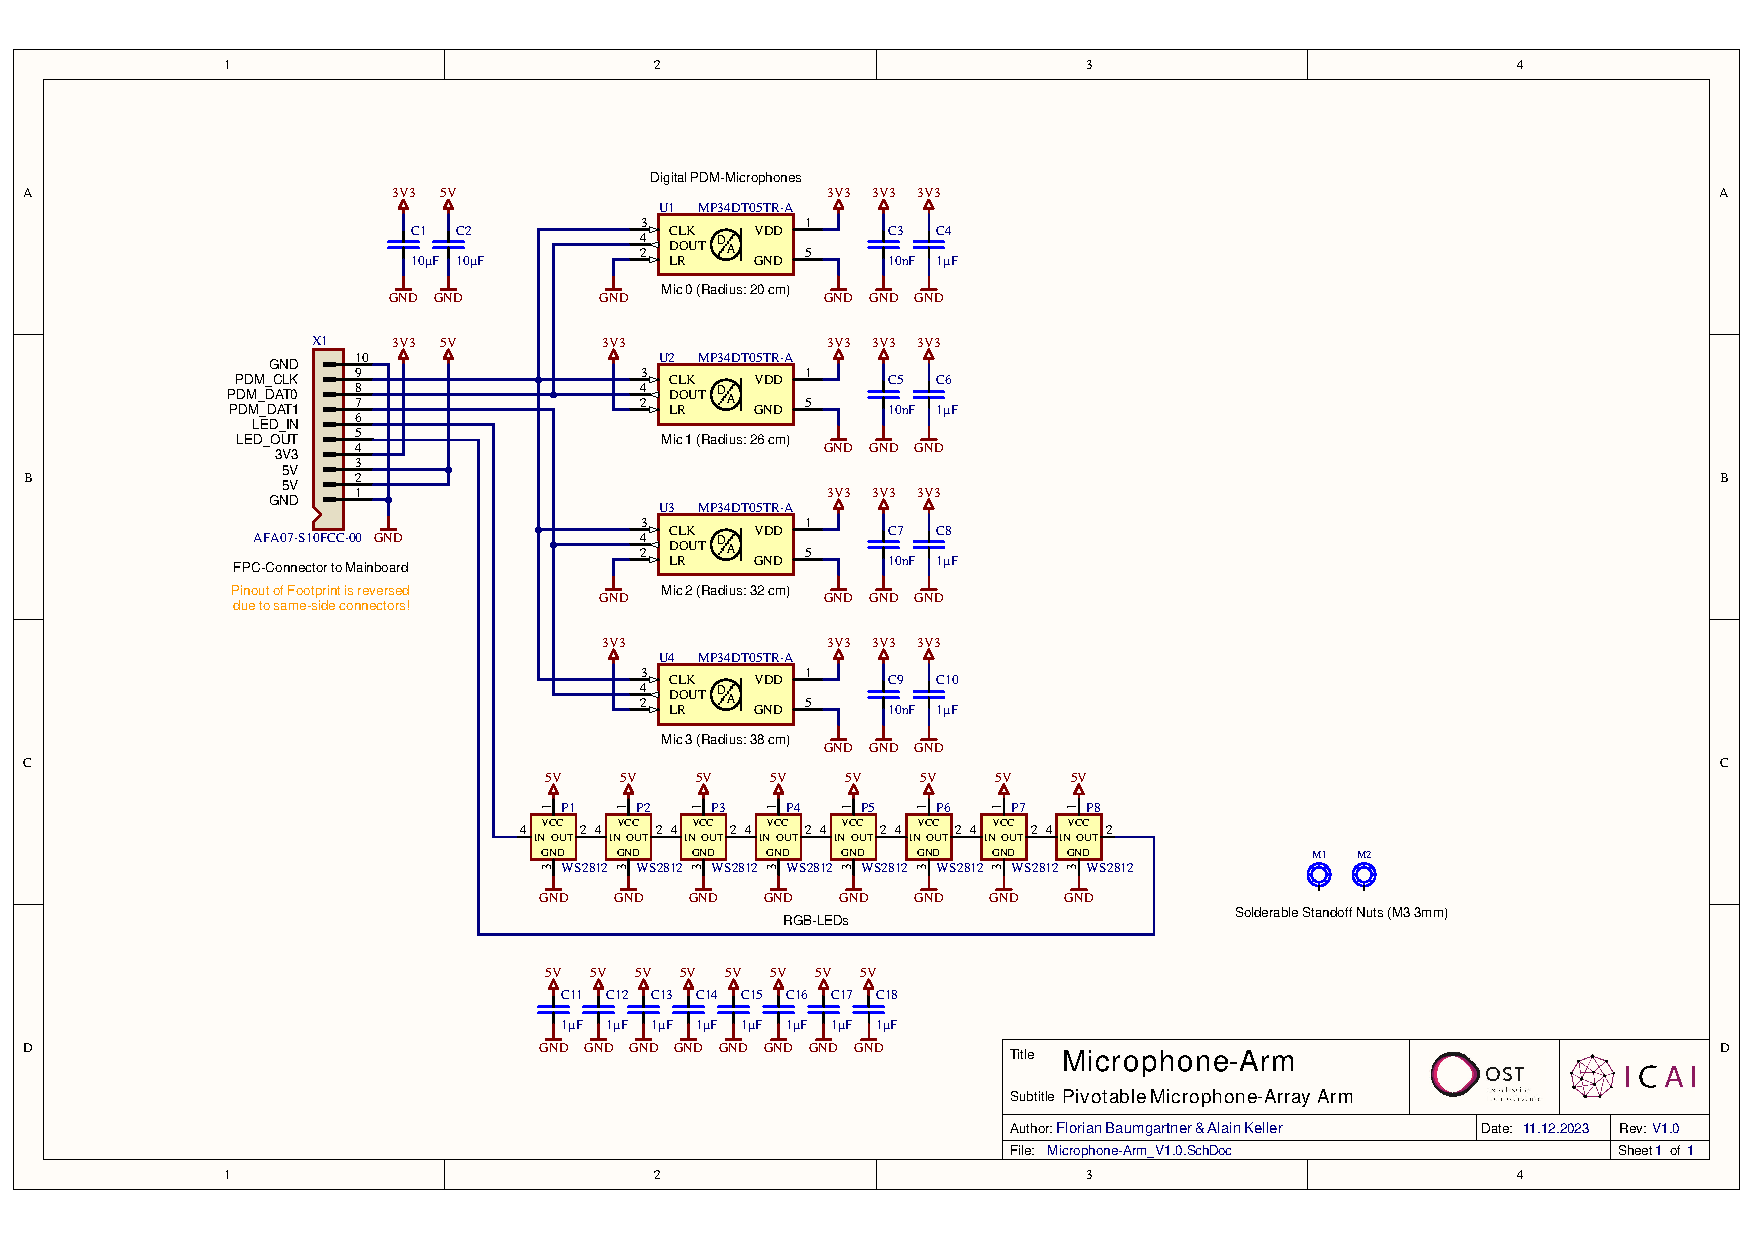
\includegraphics[angle=90, width=17.3cm, page=1]{appendix/Microphone_Arm_V1.0.pdf}}
\end{adjustwidth}
\newpage

\section{Microphone-Arm PCB Top-Layer}
\enlargethispage{2.5cm}
\begin{adjustwidth}{-0.23cm}{0cm} \hfuzz=7.0pt \vfuzz=19.0pt
	\makebox[\textwidth]{\frame{\includegraphics[angle=90, width=17.3cm, trim={0 0 0 0}, page=2]{appendix/Microphone_Arm_V1.0.pdf}}}
\end{adjustwidth}
\newpage

\section{Microphone-Arm PCB Bottom-Layer}
\enlargethispage{2.5cm}
\begin{adjustwidth}{0.23cm}{0cm} \hfuzz=7.0pt \vfuzz=19.0pt
	\makebox[\textwidth]{\frame{\includegraphics[angle=90, width=17.3cm, trim={0 0 0 0}, page=3]{appendix/Microphone_Arm_V1.0.pdf}}}
\end{adjustwidth}
\newpage

\section{Microphone-Arm PCB Top-Overlay}
\enlargethispage{2.5cm}
\begin{adjustwidth}{-0.23cm}{0cm} \hfuzz=7.0pt \vfuzz=19.0pt
	\makebox[\textwidth]{\frame{\includegraphics[angle=90, width=17.3cm, trim={0 0 0 0}, page=4]{appendix/Microphone_Arm_V1.0.pdf}}}
\end{adjustwidth}
\newpage

\section{Microphone-Arm Bill of Materials (BOM)}
\enlargethispage{2.5cm}
\begin{adjustwidth}{0.23cm}{0cm} \hfuzz=7.0pt \vfuzz=20.0pt
	\vspace{0.2cm}
	\makebox[\textwidth]{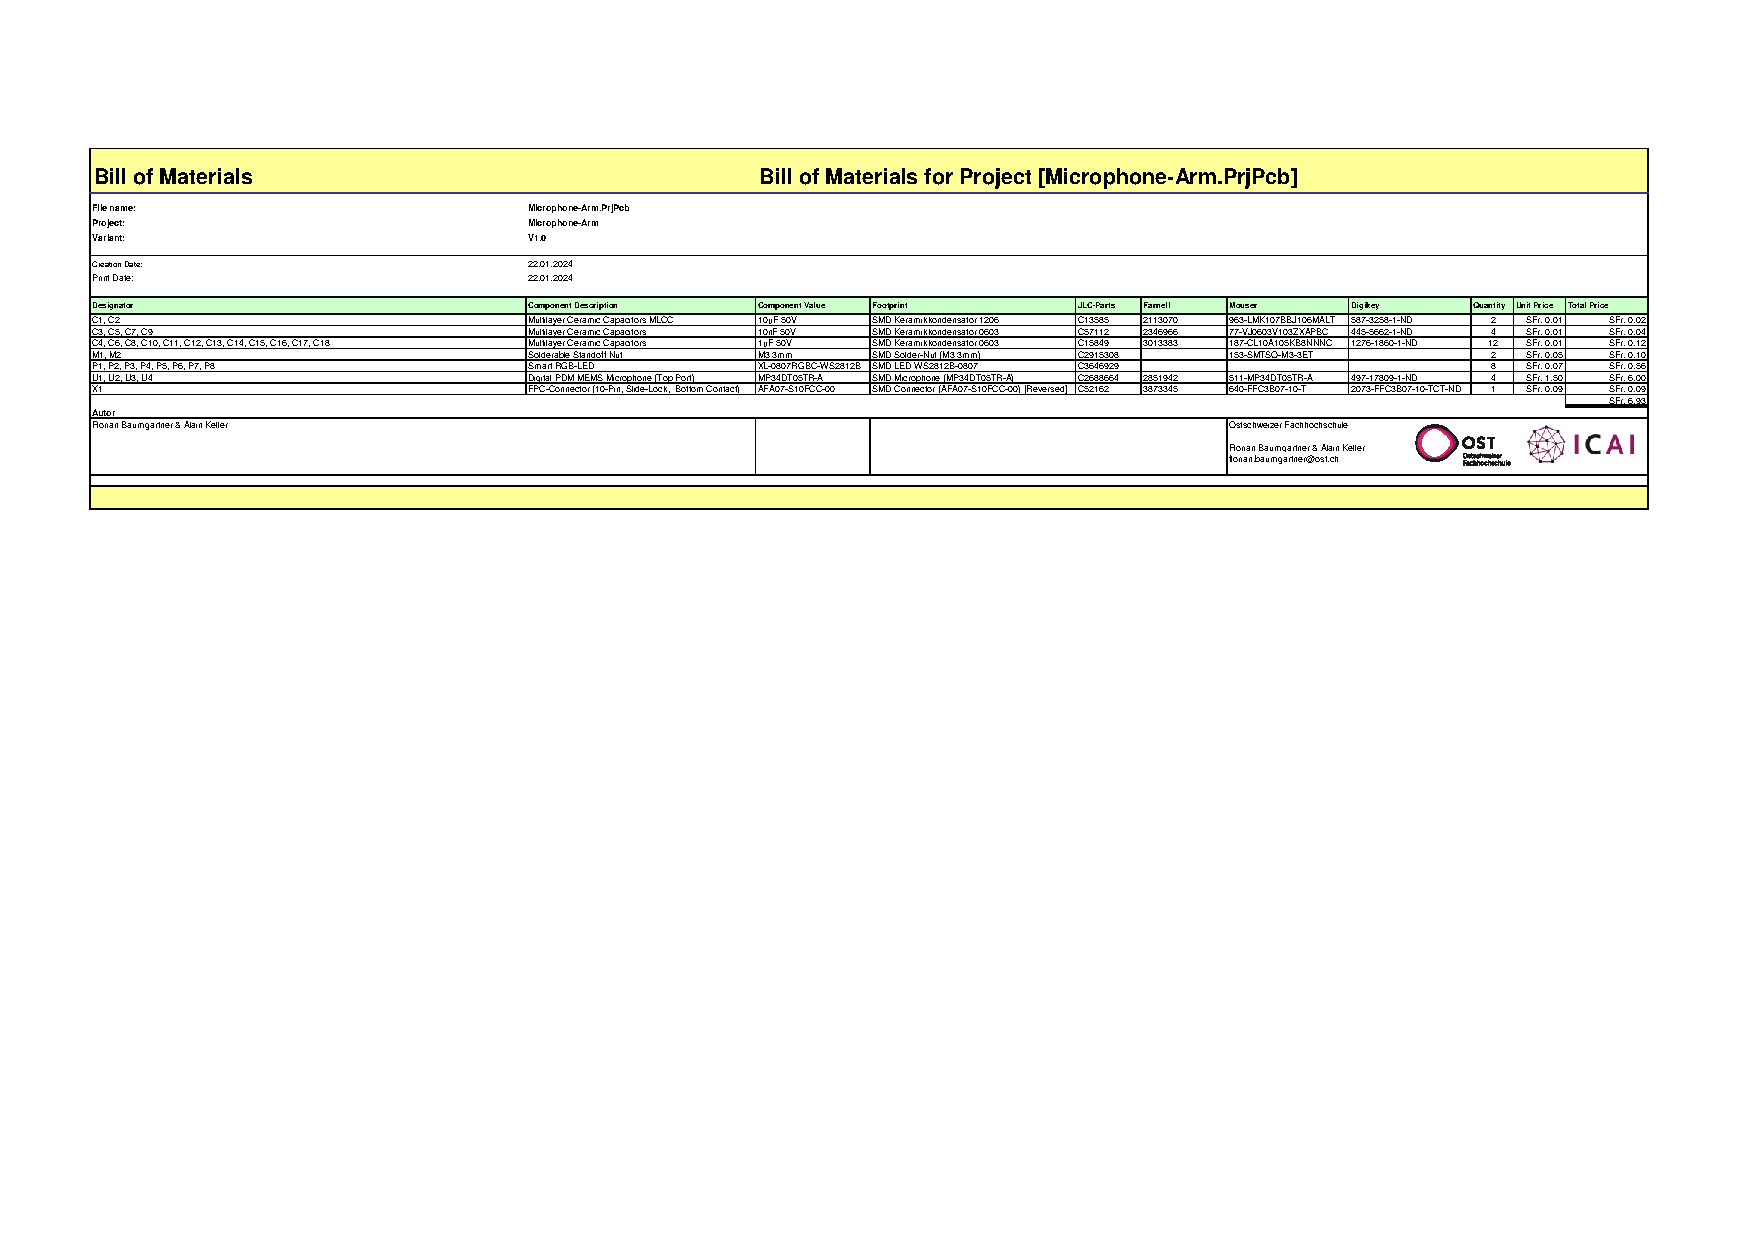
\includegraphics[angle=90, height=24.0cm]{appendix/Microphone_Arm_V1.0_BOM.pdf}}
\end{adjustwidth}
\newpage



\section{Angle-Sensor Schematics} \label{appendix_schematics_angle_sensor}
\enlargethispage{2.5cm}
\begin{adjustwidth}{-0.23cm}{0cm} \hfuzz=7.0pt \vfuzz=20.0pt
	\makebox[\textwidth]{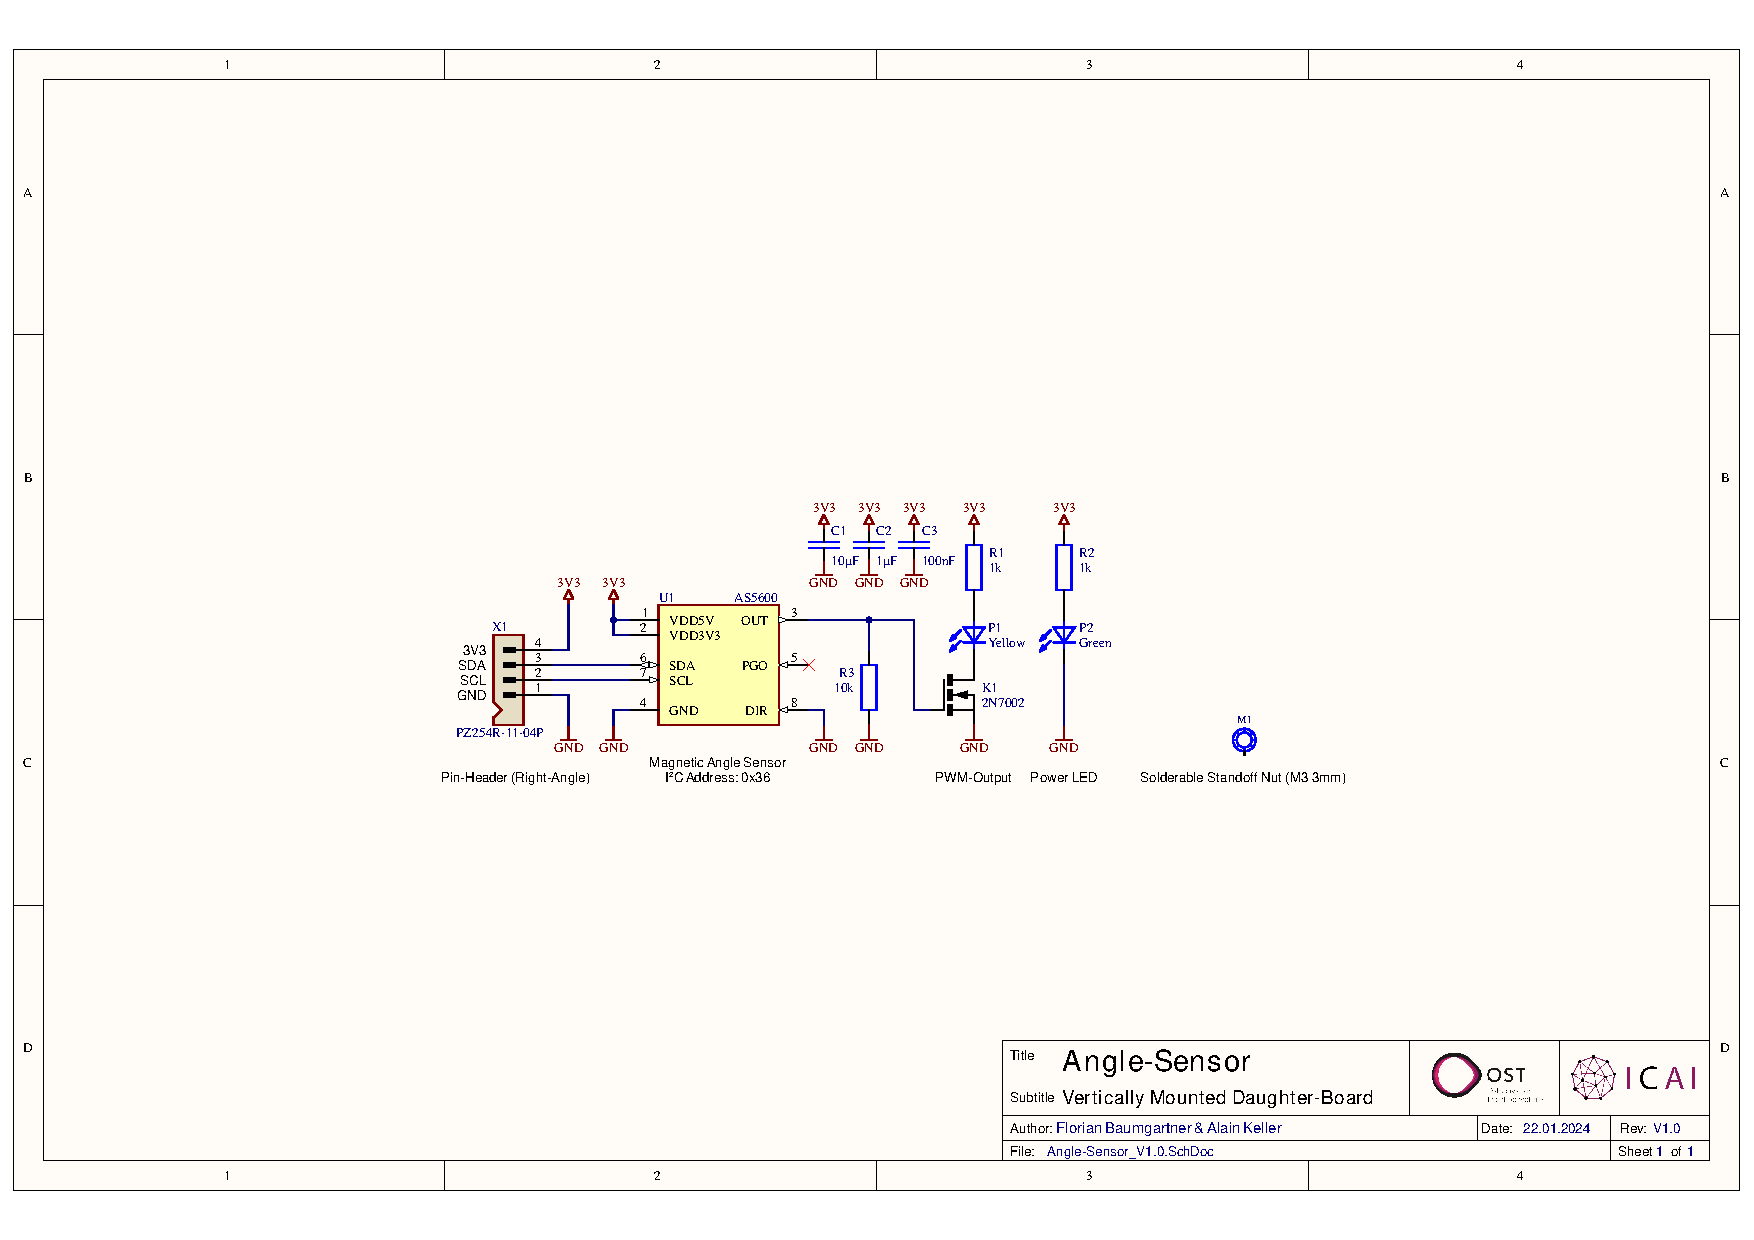
\includegraphics[angle=90, width=17.3cm, page=1]{appendix/Angle_Sensor_V1.0.pdf}}
\end{adjustwidth}
\newpage

\section{Angle-Sensor PCB Top-Layer}
\enlargethispage{2.5cm}
\begin{adjustwidth}{0.23cm}{0cm} \hfuzz=7.0pt \vfuzz=19.0pt
	\makebox[\textwidth]{\includegraphics[angle=90, width=17.3cm, trim={0.3cm 0 0.3cm 0}, page=2]{appendix/Angle_Sensor_V1.0.pdf}}
\end{adjustwidth}
\newpage

\section{Angle-Sensor PCB Bottom-Layer}
\enlargethispage{2.5cm}
\begin{adjustwidth}{-0.23cm}{0cm} \hfuzz=7.0pt \vfuzz=19.0pt
	\makebox[\textwidth]{\includegraphics[angle=90, width=17.3cm, trim={0.3cm 0 0.3cm 0}, page=3]{appendix/Angle_Sensor_V1.0.pdf}}
\end{adjustwidth}
\newpage

\section{Angle-Sensor PCB Top-Overlay}
\enlargethispage{2.5cm}
\begin{adjustwidth}{0.23cm}{0cm} \hfuzz=7.0pt \vfuzz=19.0pt
	\makebox[\textwidth]{\includegraphics[angle=90, width=17.3cm, trim={0.3cm 0 0.3cm 0}, page=4]{appendix/Angle_Sensor_V1.0.pdf}}
\end{adjustwidth}
\newpage

\section{Angle-Sensor PCB Bottom-Overlay}
\enlargethispage{2.5cm}
\begin{adjustwidth}{-0.23cm}{0cm} \hfuzz=7.0pt \vfuzz=19.0pt
	\makebox[\textwidth]{\includegraphics[angle=90, width=17.3cm, trim={0.3cm 0 0.3cm 0}, page=5]{appendix/Angle_Sensor_V1.0.pdf}}
\end{adjustwidth}
\newpage

\section{Angle-Sensor PCB Outline}
\enlargethispage{2.5cm}
\begin{adjustwidth}{0.23cm}{0cm} \hfuzz=7.0pt \vfuzz=19.0pt
	\makebox[\textwidth]{\includegraphics[angle=90, width=17.3cm, trim={0.3cm 0 0.3cm 0}, page=6]{appendix/Angle_Sensor_V1.0.pdf}}
\end{adjustwidth}
\newpage

\section{Angle-Sensor Bill of Materials (BOM)}
\enlargethispage{2.5cm}
\begin{adjustwidth}{-0.23cm}{0cm} \hfuzz=7.0pt \vfuzz=20.0pt
	\vspace{0.2cm}
	\makebox[\textwidth]{\includegraphics[angle=90, height=24.0cm]{appendix/Angle_Sensor_V1.0_BOM.pdf}}
\end{adjustwidth}
\newpage



\section{Mechanical Drawing of Main Mounting Pole} \label{appendix_mechanical_drawing_main_mounting_pole}
\enlargethispage{2.5cm}
\begin{adjustwidth}{0.23cm}{0cm} \hfuzz=7.0pt \vfuzz=20.0pt
	\makebox[\textwidth]{\frame{\includegraphics[angle=90, width=17.3cm, page=3]{appendix/Mechanical_Drawings.pdf}}}
\end{adjustwidth}
\newpage

\section{Mechanical Drawing of Top Mounting Ring} \label{appendix_mechanical_drawing_top_mounting_ring}
\enlargethispage{2.5cm}
\begin{adjustwidth}{-0.23cm}{0cm} \hfuzz=7.0pt \vfuzz=20.0pt
	\makebox[\textwidth]{\frame{\includegraphics[angle=90, width=17.3cm, page=1]{appendix/Mechanical_Drawings.pdf}}}
\end{adjustwidth}
\newpage

\section{Mechanical Drawing of Bottom Sliding Ring} \label{appendix_mechanical_drawing_bottom_sliding_ring}
\enlargethispage{2.5cm}
\begin{adjustwidth}{0.23cm}{0cm} \hfuzz=7.0pt \vfuzz=20.0pt
	\makebox[\textwidth]{\frame{\includegraphics[angle=90, width=17.3cm, page=2]{appendix/Mechanical_Drawings.pdf}}}
\end{adjustwidth}
\newpage

\section{Mechanical Drawing of Antenna Top Mount} \label{appendix_mechanical_drawing_antenna_top_mount}
\enlargethispage{2.5cm}
\begin{adjustwidth}{-0.23cm}{0cm} \hfuzz=7.0pt \vfuzz=20.0pt
	\makebox[\textwidth]{\frame{\includegraphics[angle=90, width=17.3cm, page=4]{appendix/Mechanical_Drawings.pdf}}}
\end{adjustwidth}
\newpage

\section{Mechanical Drawing of Antenna Bottom Mount} \label{appendix_mechanical_drawing_antenna_bottom_mount}
\enlargethispage{2.5cm}
\begin{adjustwidth}{0.23cm}{0cm} \hfuzz=7.0pt \vfuzz=20.0pt
	\makebox[\textwidth]{\frame{\includegraphics[angle=90, width=17.3cm, page=5]{appendix/Mechanical_Drawings.pdf}}}
\end{adjustwidth}
\newpage

\section{Mechanical Drawing of Antenna Pole} \label{appendix_mechanical_drawing_antenna_pole}
\enlargethispage{2.5cm}
\begin{adjustwidth}{-0.23cm}{0cm} \hfuzz=7.0pt \vfuzz=20.0pt
	\makebox[\textwidth]{\frame{\includegraphics[angle=90, width=17.3cm, page=6]{appendix/Mechanical_Drawings.pdf}}}
\end{adjustwidth}
\newpage
